
\begin{figure}[h]\centering
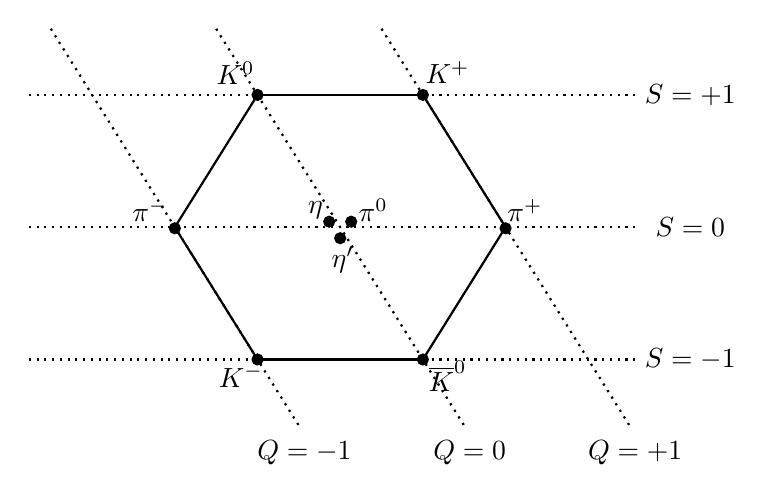
\begin{tikzpicture}
\begin{scope}[scale = 0.7] % overall scale 
%%
\begin{scope}[yscale = 1.2]
%%
%% hjelpelinjer
\draw    [thick, dotted]  (0,0)  --  (11,0);
\draw    [thick,dotted]  (0,2)  --  (11,2);
\draw    [thick, dotted]  (0,4)  --  (11,4);
\draw    [thick, dotted]  (0.4,5)  --  (4.9,-1);
\draw    [thick, dotted]  (0.4+3,5)  --  (4.9+3,-1);
\draw    [thick, dotted]  (0.4+6,5)  --  (4.9+6,-1);
%% hexagon
\begin{scope}[xshift = 0.05cm] % scope skifter og/eller skalerer innmaten
\draw    [thick]  (4.1,4)  --  (7.1,4);
\draw    [thick]  (4.1,4)  --  (2.6,2);
\draw    [thick]  (7.1,4)  --  (8.6,2);
\draw    [thick]  (4.1+4.5,2)  --  (2.6+4.5,0);
\draw    [thick]  (7.1-4.5,2)  --  (8.6-4.5,0);
\draw    [thick]  (4.1,0)  --  (7.1,0);
\end{scope}
\end{scope}
%% dots
\draw [fill] (4.15,0) circle [radius=0.1];
\draw [fill] (4.15+3,0) circle [radius=0.1];
\draw [fill] (4.15,4.8) circle [radius=0.1];
\draw [fill] (4.15+3,4.8) circle [radius=0.1];
\draw [fill] (2.65,2.38) circle [radius=0.1];
\draw [fill] (2.65+6,2.38) circle [radius=0.1];
\begin{scope}[xshift = -1.3cm,yshift = 0.7cm]
\draw [fill] (2.65+4.1,1.8) circle [radius=0.1];
\draw [fill] (2.65+4.5,1.8) circle [radius=0.1];
\draw [fill] (2.65+4.3,1.5) circle [radius=0.1];
\end{scope}
%% S,Q
\node at (12,0) {$S = -1$};
\node at (12,2.4) {$S = 0$};
\node at (12,4.8) {$S = +1$};
\node at (5,-1.7) {$Q = -1$};
\node at (5+3,-1.7) {$Q = 0$};
\node at (5+6,-1.7) {$Q = +1$};
%%partikler
\node at (4.15-0.3,0-0.3) {$K^-$};
\node at (4.15+3+0.45,0-0.3) {$\overline{K}^0$};
\node at (4.15-0.4,0-0.3 +5.5) {$K^0$};
\node at (4.15+3+0.45,0-0.3+5.5) {$K^+$};
\node at (2.2,2.7) {$\pi^-$};
\node at (2.2+6.8,2.7) {$\pi^+$};
\node at (5.2,2.7) {$\eta$};
\node at (6.25,2.7) {$\pi^0$};
\node at (5.7,1.8) {$\eta'$};
%%
%%
\end{scope} % overall scale end
\end{tikzpicture}
\caption{The pseudoscalar meson nonet}
\end{figure}

